\chapter{Bilan}

\section{Bilan du travail r\'ealis\'e}

Ce bilan r\'esumera le travail r\'ealis\'e durant le stage.
Dans une premi\`ere partie, un r\'ecapitulatif du projet sera donn\'e, avec notamment un graphique afin de montrer les fonctionnalit\'es reprises de {\Yuukou} ainsi que les diff\'erentes fonctionnalit\'es qu'apporte {\YuukouII}.
Ensuite le calendrier des 16 semaines de stage, avec les diff\'erentes t\^aches effectu\'ees semaines apr\`es semaines.
Il sera suivi par une partie donnant ce qu'apporte le projet \`a l'Universit\'e, les avantages qu'elle peut en tirer.
Enfin une derni\`ere partie traitera des am\'eliorations qu'il est possible d'apporter au service Web afin d'accro\^itre ses performances et ses fonctionnalit\'es.

\subsection{R\'ecapitulatif du projet}

La figure~\ref{figure:yuukouEtYuukouII} permet de donner une vue d'ensemble sur les principales fonctionnalit\'es dont le projet dispose.
Les cadres pleins repr\'esentent des fonctionnalit\'es dont le principe a \'et\'e repris de {\Yuukou}, les cadres en pointill\'es, quant \`a eux, repr\'esentent les nouvelles fonctionnalit\'es qu'apporte \YuukouII.

\clearpage

\begin{figure}[!ht]
	\centering
	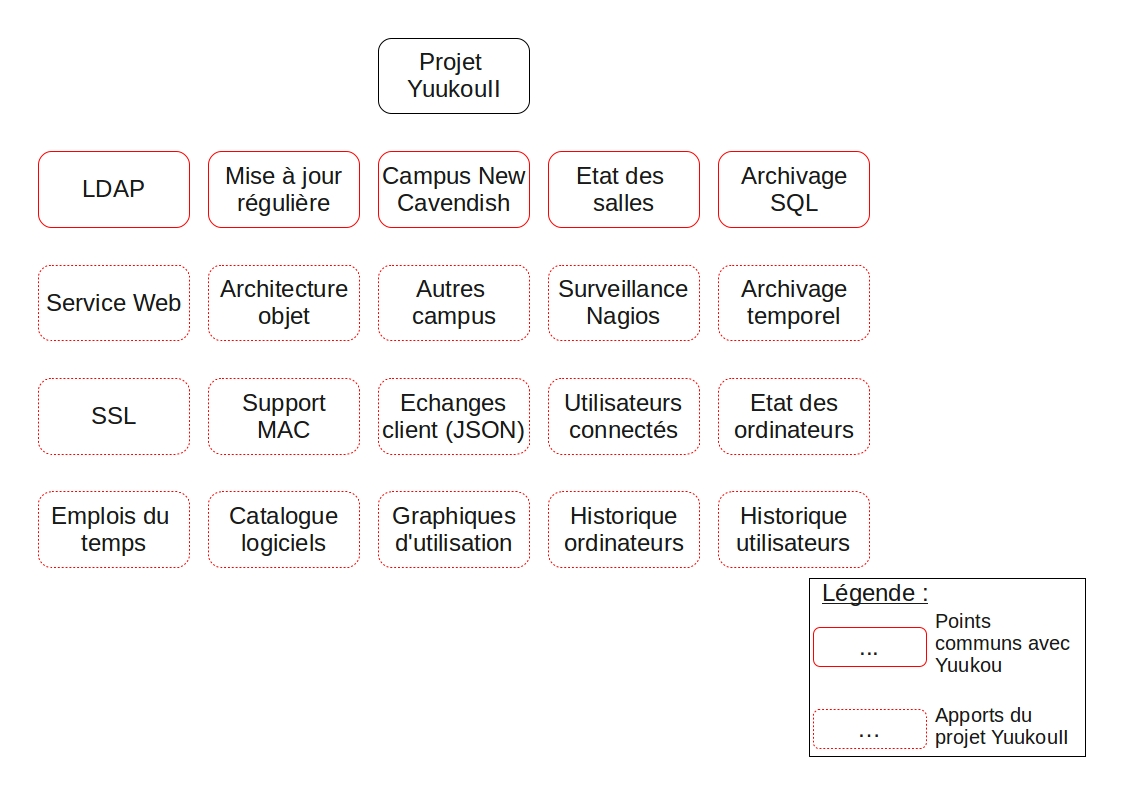
\includegraphics[scale=0.375]{yuukouEtYuukouII.jpg}
	\caption{R\'ecapitulatif des fonctionnalit\'es reprises de {\Yuukou} et les nouvelles de \YuukouII}
	\label{figure:yuukouEtYuukouII}

\end{figure}

\subsection{Calendrier du stage}

Voici le calendrier du stage d'une dur\'ee de 16 semaines commen\c{c}ant le 13 f\'evrier 2012 et terminant le 4 juin 2012.
Certains points ont demand\'e plus de travail que d'autres, comme la conception du cycle principal du service Web ou encore la mise en place du SSL qui a pos\'ee quelques difficult\'es.

\begin{description}
	\item[semaine 1] : Arriv\'ee et d\'ecouverte du projet, premier entretien avec l'\'equipe technique et leurs attentes;
	\item[semaine 2] : D\'ecouverte des services Web et choix des outils utilis\'es;
	\item[semaine 3 et 4] : Conception de la base de donn\'ees et impl\'ementation du cycle principal de l'application;
	\item[semaine 5] : Mise en place de l'emploi du temps et d\'ebut mise en place de SSL;
	\item[semaine 6] : Mise en place du syst\`eme JSON et fin de mise en place de SSL;
	\item[semaine 7 et 8] : D\'eveloppement des m\'ethodes Web;
	\item[semaine 9] : Mise en place de l'architecture finale et d\'eveloppement des m\'ethodes Web;
	\item[semaine 10] : D\'ebut de r\'edaction du rapport (pr\'esentation et sujet);
	\item[semaine 11] : D\'eveloppement des m\'ethodes Web;
	\item[semaine 12 et 13] : R\'ecup\'eration du catalogue de logiciels de M\'ediaWiki;
	\item[semaine 14] : Ajout de m\'ethodes Web et am\'elioration du syst\`eme de chargement de la base de donn\'ees;
	\item[semaine 15] : R\'edaction du rapport de stage et maintenance des fonctionnalit\'es du service Web;
	\item[semaine 16] : Fin d'\'ecriture du rapport de stage.

\end{description}

\subsection{Bilan pour l'Universit\'e}

Le service Web est fonctionnel \`a l'Universit\'e.
Il dispose d'un cycle principal permettant la r\'ecup\'eration des donn\'ees de Nagios et le stockage dans la base de donn\'ees.
De nombreuses fonctionnalit\'ees ont \'et\'e d\'evelopp\'ees pour \'etendre les possibilit\'es du service Web.
Une s\'ecurisation des communications avec la mise en place du protocole SSL.
Une gestion des emplois du temps en r\'ecup\'erant quotidiennement les diff\'erents emplois du temps des campus de l'Universit\'e.
Une gestion de la configuration logicielle des salles informatiques avec l'extraction des donn\'ees pr\'esentes sur le \textit{MediaWiki} de la \textit{School of Electronics and Computer Science}.
Une g\'en\'eration d'un graphe d'utilisation des salles informatiques dans une p\'eriode donn\'ee.

Le service Web dispose de nombreuses fonctions permettant \`a un client de r\'ecup\'erer juste les informations dont il a besoin concernant la disponibilit\'e des salles en temps r\'eel.
Mais aussi les historiques dans le temps des connexions.
Il propose aussi une gestion de cycle permettant de l'arr\^eter et de le remettre en marche.

L'utilisation de JSON permet la cr\'eation de client ind\'ependamment du langage employ\'e.
Une fois la structure du fichier retourn\'e comprise, il est facile d'extraire les donn\'ees voulues et de les afficher.

Ajout\'e \`a cela la documentation Java (\textit{javadoc}) du service Web afin que dans le futur diff\'erentes am\'eliorations, parmi celles exprim\'ees au \S~\ref{section:amelioration}, soient mises en place.

\subsection{Am\'eliorations possibles}
\label{section:amelioration}

Le projet {\YuukouII} est loin d'\^etre fini m\^eme si fonctionnel \`a l'heure actuelle.
Il reste diverses fonctionnalit\'es \`a d\'evelopper.
Une de ces fonctionnalit\'es serait de rajouter une s\'ecurit\'e lors de l'acc\`es aux m\'ethodes du service Web par le client.
En effet, il serait int\'eressant que le client s'authentifie.
De ce fait, deux r\^oles pourraient \^etre d\'efinis : administrateur et utilisateur.
Avec cette m\'ethode, un utilisateur ne pourrait jamais se servir d'une m\'ethode dite priv\'ee car actuellement, si un client d\'eveloppe son propre programme pour acc\'eder au service Web {\YuukouII}, une fois le protocole SSL en place, rien ne l'emp\^eche d'utiliser les fonctions qu'il veut.

Des am\'eliorations peuvent aussi \^etre port\'ees sur la fa\c{c}on dont RRDtool a \'et\'e mis en place.
Il ne s'agit que d'un essai pour tester les possibilit\'es, mais il serait int\'eressant de l'int\'egrer pleinement au service Web et surtout au cycle principal d'ex\'ecution.
De ce fait, les donn\'ees seraient enregistr\'ees en temps r\'eel et les requ\^etes de g\'en\'eration de graphe pourraient gagner en rapidit\'e d'ex\'ecution.
De plus, cette m\'ethode rendrait une utilisation normale de RRDtool au service Web.

La suite concernerait les attentes pour les emplois du temps et le catalogue logiciels.
En effet, la gestion des emplois du temps est susceptible d'\'evoluer vers une notation plus lisible des salles par le service responsable de la cr\'eation des emplois du temps.
Cela permettrait un suivi de toutes les salles informatiques au lieu de seulement certaines actuellement situ\'ees \`a la \textit{School of Electronics and Computer Science}.
Pour le catalogue de logiciels, le principe est un peu le m\^eme.
Ne concernant que la \textit{School of Electronics and Computer Science}, il serait int\'eressant de trouver une fa\c{c}on simple de r\'ecup\'erer les informations sur la configuration logicielle des autres salles.
Par exemple, si une partie de la base de donn\'ees permettant de construire cette configuration, en amont, pouvait \^etre disponible, l'extraction des donn\'ees s'en verrait simplifi\'ee et plus compl\`ete du fait qu'elle serait effective pour toutes les salles surveill\'ees par Nagios.

Il pourrait aussi \^etre impl\'ement\'e une s\'erie de petites fonctions permettant d'effectuer des modifications d'informations, quand le service Web est en maintenance, sur les diff\'erentes tables.
Par exemple l'ajout d'une salle avec l'aide d'une interface Web.

Nagios surveille actuellement les salles informatiques de l'Universit\'e, cependant, il est possible de lui faire surveiller les imprimantes et d'ajouter les services adapt\'es comme la gestion du niveau d'encre et du papier.
Un \'etudiant recherchant une imprimante de libre obtiendrait les salles correspondantes.
Avec cela, il serait possible d'avoir un statut complet d'une salle informatique.

Il serait aussi int\'eressant d'ajouter des fonctions au service Web pour retourner les informations sur la surveillance des salles sous forme d'un flux RSS$^*$ pouvant \^etre exploit\'e de fa\c{c}on diff\'erente par un client.


\section{Bilan personnel}

D'un point de vue humain, ce stage m'a beaucoup apport\'e, sp\'ecialement au niveau de la langue.
Je me suis rendu compte combien il est difficile au d\'ebut de communiquer convenablement avec quelqu'un.
Le m\^eme cycle se r\'ep\`ete : on essaye de traduire ce que l'on entend, ensuite on r\'efl\'echi \`a la r\'eponse en fran\c{c}ais, on la traduit rapidement et on la dit plus ou moins bien.
C'est compliqu\'e de se d\'efaire de ce cycle mais apr\`es quelques mois, j'ai pu ressentir beaucoup plus de facilit\'e \`a communiquer avec les membres du CPC.

De plus, je suis vraiment content d'avoir pu effectuer mon stage dans une ville si cosmopolite que Londres.
J'ai pu y d\'ecouvrir une vie un peu diff\'erente de celle que je connaissais.
Durant les quatre mois, j'ai r\'esid\'e dans une r\'esidence \'etudiante o\`u j'ai partag\'e une chambre avec un croate, de ce fait, je n'avais pas d'autre choix que de parler anglais avec lui.
C'\'etait d'autant plus le cas que la majorit\'e des r\'esidents n'\'etaient pas anglais, mais venaient d'un peu partout dans le monde.
Chose qui, je pense, m'a beaucoup fait progresser notamment dans le parl\'e, tout en gardant quand m\^eme un fort accent fran\c{c}ais.

Concernant le cadre du stage, j'ai beaucoup appr\'eci\'e la prise en charge de M. DELAITRE qui s'est beaucoup impliqu\'e dans ce projet, tant dans la partie service Web que dans la partie affichage.
J'ai r\'eellement aim\'e la libert\'e d'action qu'il m'a laiss\'e dans le projet tout en fixant les objectifs qu'il voulait voir accompli.

La collaboration avec les diff\'erents acteurs du projet d'affichage s'est tr\`es bien pass\'ee, notamment avec M. Yacine MAGHEZZI comme nous \'etions dans le m\^eme bureau.
Nous avons d\^u beaucoup discuter l'un avec l'autre concernant le retour d'informations du service Web.
Mon objectif \'etait vraiment de faciliter un maximum le travail des autres d\'eveloppeurs pour qu'ils puissent se concentrer essentiellement sur la partie affichage.

D'un point de vue p\'edagogique, ce stage fut vraiment tr\`es riches en nouvelles connaissances.
J'ai pu y d\'ecouvrir les services Web que je ne connaissais pas auparavant ainsi que des outils qui m'\'etaient totalement inconnus comme NetBeans et GlassFish.
J'avoue avoir des appr\'ehensions quand on me parle de technologies du Web mais le projet que m'a confi\'e M. Thierry DELAITRE m'a vraiment passionn\'e du d\'ebut \`a la fin du stage.
J'ai pu r\'eutiliser beaucoup de mes acquis avec le d\'eveloppement Java, les interactions avec les bases de donn\'ees ou encore la manipulation de fichiers XML.



\clearpage
